\documentclass[12pt,a4paper,twoside,openright]{book}
\usepackage[T1]{fontenc}
\usepackage[utf8]{inputenc}
\usepackage{lmodern}
\usepackage[english]{babel}
\usepackage{geometry}
\geometry{a4paper,left=2.5cm,right=2.5cm,top=2.7cm,bottom=2.5cm}
\usepackage{graphicx}
\usepackage{amsmath,amssymb}
\usepackage{booktabs,longtable,array}
\usepackage{microtype}
\usepackage[hidelinks]{hyperref}
\usepackage{xurl}
\usepackage{enumitem}
\setlength{\parindent}{0pt}
\setlength{\parskip}{0.65em}
\setlength{\emergencystretch}{3em}
\setcounter{secnumdepth}{2}
\setcounter{tocdepth}{2}
\renewcommand{\bibname}{Bibliography}
\newcommand{\maxwidth}{\linewidth}
\newcommand{\maxheight}{0.78\textheight}
\setkeys{Gin}{width=\maxwidth,height=\maxheight,keepaspectratio}
\providecommand{\tightlist}{\setlength{\itemsep}{0pt}\setlength{\parskip}{0pt}}

\begin{document}
\frontmatter
\begin{titlepage}
\thispagestyle{empty}
\begin{center}
\vspace*{0.8cm}

\includegraphics[width=7.0cm]{media/extract-000.png}\\[0.2cm]
{\large Department 4: Computer Science}\par
\vspace{4.2cm}
{\LARGE Do Macroeconomic Covariates Improve Foundation-Model Portfolios?\par}
\vspace{0.45cm}
{\Large Evidence from Chronos-2 and U.S. Sector ETFs\par}
\end{center}
\vfill
\begin{minipage}{0.72\textwidth}
{\Large Master's Research Paper\\
 in the study program Web and Data Science}\par
\vspace{1.0cm}
submitted by\\[0.45cm]

{\Large\textbf{Iqra Afzaal}}\par
Matriculation No.: 225100299\par

\vspace{0.4cm}

{\Large\textbf{Amna Muzaffar}}\par
Matriculation No.: 224201174\par

\vspace{0.9cm}
\textbf{First Examiner:} [Name]\\
\textbf{Second Examiner:} [Name, if applicable]\par
\vspace{0.9cm}
Koblenz, September 2026
\end{minipage}
\end{titlepage}

\chapter*{Abstract}
\addcontentsline{toc}{chapter}{Abstract}
This study examines whether macroeconomic covariates improve the practical value of zero-shot time-series foundation-model forecasts in portfolio construction. The central question is not only whether external variables reduce forecast error, but whether any statistical improvement survives the nonlinear transformation from forecasts to portfolio weights and ultimately produces economically better investment outcomes. A controlled predict-then-optimize experiment is implemented with Chronos-2 on 11 U.S. sector exchange-traded funds over a 2023--2026 evaluation period. Three forecasting arms are compared: a price-only baseline (Arm B), a model supplied with historical macroeconomic covariates (Arm A), and an extension that first forecasts future macroeconomic paths and supplies them as future covariates (Arm C). The macro variables are VIX volatility, the U.S. 10-year Treasury yield, WTI crude oil, gold, and the U.S. dollar index. Forecasts use information available through each decision date and predict the next 21 trading days; the portfolio holding horizon is aligned to the same 21-day interval. Historical covariates improve several forecast-error measures relative to the no-covariate baseline. In the portfolio experiment, Arm A achieves a cumulative return of 65.36\% and an annualized Sharpe ratio of 1.098, compared with 44.92\% and 0.839 for Arm B. However, the paired circular block-bootstrap confidence interval for the Sharpe difference includes zero (difference 0.264; 95\% CI [-0.202, 0.735]; p=0.2396), so the economic improvement is not statistically conclusive.

\textbf{Keywords:} time-series foundation models, Chronos-2, macroeconomic covariates, portfolio optimization, zero-shot forecasting, sector ETFs, Sharpe ratio

\chapter*{Zusammenfassung}
\addcontentsline{toc}{chapter}{Zusammenfassung}
Diese Arbeit untersucht, ob makroökonomische Kovariaten den praktischen Nutzen von Zero-Shot-Prognosen eines Time-Series-Foundation-Models für die Portfoliokonstruktion verbessern. Im Mittelpunkt steht nicht nur die Frage, ob externe Variablen den Prognosefehler reduzieren, sondern ob sich statistische Verbesserungen auch in ökonomisch besseren Portfolioergebnissen niederschlagen. Dazu wird ein kontrolliertes Predict-then-Optimize-Experiment mit Chronos-2 auf elf US-Sektor-ETFs im Evaluationszeitraum 2023 bis 2026 durchgeführt. Verglichen werden ein Preis-Basismodell ohne Kovariaten (Arm B), ein Modell mit historischen makroökonomischen Kovariaten (Arm A) sowie eine Erweiterung mit prognostizierten zukünftigen Makropfaden (Arm C).

\chapter*{Declaration}
\addcontentsline{toc}{chapter}{Declaration}
I hereby declare that I have formulated the present thesis independently and have not used any sources or aids other than those explicitly stated. The thesis has not been presented to any other examination board in the same or a similar form. All statements that have been taken over literally or analogously are marked as such.

\vspace{1.5cm}
I agree to the inclusion of this thesis in the library. \hfill yes $\square$\quad no $\square$\\[0.5cm]
I consent to the publication of this thesis on the Internet. \hfill yes $\square$\quad no $\square$

\vfill
Koblenz, September 2026 \hfill (Signature)
\cleardoublepage
\tableofcontents
\cleardoublepage
\chapter*{List of Abbreviations}
\addcontentsline{toc}{chapter}{List of Abbreviations}
\begin{tabular}{ll}
ETF & Exchange-Traded Fund\\
FM & Foundation Model\\
TSFM & Time-Series Foundation Model\\
VIX & CBOE Volatility Index\\
WTI & West Texas Intermediate crude oil\\
MAPE & Mean Absolute Percentage Error\\
MAE & Mean Absolute Error\\
RMSE & Root Mean Squared Error\\
IC & Information Coefficient\\
MV & Mean-Variance\\
EW & Equal Weight\\
CI & Confidence Interval
\end{tabular}
\cleardoublepage
\mainmatter
\chapter{Introduction}\label{introduction}

\section{Motivation}\label{motivation}

Forecasting financial markets is difficult because the signal of
interest is weak relative to noise, relationships change across market
regimes, and a model that performs well on a statistical loss does not
necessarily create value after forecasts are translated into investment
decisions. These difficulties make financial forecasting a demanding
test for modern machine-learning systems. At the same time, the
emergence of time-series foundation models has changed the practical
forecasting workflow. Instead of training a new model for every asset
and horizon, a pretrained model can be applied zero-shot to previously
unseen series. Chronos and its successor Chronos-2 are examples of this
paradigm. Chronos-2 extends the foundation-model idea from univariate
forecasting to multivariate and covariate-informed forecasting, allowing
external variables to enter the model without task-specific retraining.

The possibility of conditioning a pretrained forecaster on external
information is particularly relevant for finance. Asset prices do not
evolve in isolation. Equity sectors can respond differently to
volatility, interest rates, commodity prices, and currency conditions.
Energy-related sectors may be sensitive to oil; rate-sensitive sectors
can react to changes in Treasury yields; the VIX can proxy market-wide
risk aversion; gold can reflect defensive demand and inflation concerns;
and the U.S. dollar can affect multinational firms and global financial
conditions. A sufficiently flexible nonlinear forecaster may be able to
use these variables in ways that simple linear predictive regressions
cannot.

Yet a forecasting improvement is not the same as an investment
improvement. A portfolio optimizer acts on relative expected returns,
risk estimates, constraints, and transaction costs. Small forecast
changes can produce large reallocations when they alter the
cross-sectional ranking of assets, while a lower average forecast error
may have little portfolio effect if it occurs on observations that do
not change portfolio weights. Conversely, a statistically modest
improvement can matter economically when it consistently improves the
ranking of investable assets. This distinction motivates the present
study.

\section{Problem Statement and Research
Questions}\label{problem-statement-and-research-questions}

Prior research provides two pieces of evidence that are individually
important but not yet fully connected. First, covariates can improve
forecasting when the model is sufficiently flexible. Gu, Kelly, and Xiu
(2020), for example, show that nonlinear machine-learning methods can
exploit rich predictor interactions and generate economic gains in
asset-pricing applications. More recently, ChronosX demonstrates that
pretrained time-series models can be adapted to use exogenous variables,
and Chronos-2 directly supports past and future covariates. Second,
recent studies show that foundation-model forecasts can be incorporated
into financial strategies, including long/short stock portfolios,
factor-selection systems, and portfolio reinforcement learning. The
missing link is a controlled test of whether adding macroeconomic
covariates to a zero-shot foundation model changes not only forecast
accuracy but also the value of a multi-asset portfolio.

The main research question is therefore: Do macroeconomic covariates
improve the economic value of zero-shot Chronos-2 forecasts when those
forecasts are used in a fixed portfolio-construction pipeline?

This question is decomposed into four empirical sub-questions. RQ1 asks
whether historical macroeconomic covariates improve out-of-sample
forecast accuracy relative to a price-only Chronos-2 baseline. RQ2 asks
whether any forecast improvement translates into higher portfolio return
or risk-adjusted performance under the same mean-variance allocation
rule. RQ3 asks whether explicitly forecasting the future macroeconomic
path and providing it as future covariates adds value beyond historical
covariates alone. RQ4 asks which individual covariates appear most
important for the observed portfolio results.

\section{Contributions}\label{contributions}

The study makes four practical contributions. First, it constructs a
controlled on/off covariate experiment in which the core forecasting
model and portfolio rule are held fixed. This isolates the role of the
information set more cleanly than comparisons across different
forecasting architectures. Second, it aligns the information cutoff,
forecast horizon, expected-return definition, and realized holding
period. At each decision date t, the model sees information available
through t, forecasts t+1 through t+21, and the portfolio is evaluated
over exactly the same 21-trading-day interval. Third, the evaluation
combines conventional forecast metrics with return-oriented measures,
cross-sectional rank information, portfolio outcomes, and
time-series-aware bootstrap inference. Fourth, the
leave-one-covariate-out experiment examines whether the aggregate effect
of covariates is concentrated in particular macro variables.

The contribution is deliberately narrower than claiming a new
forecasting architecture. Chronos-2 is used as a frozen pretrained
model, and the portfolio optimizer is a conventional long-only
mean-variance rule. The novelty lies in connecting covariate-informed
zero-shot forecasting to multi-asset economic evaluation under a
controlled and reproducible design.

\section{Structure of the Paper}\label{structure-of-the-paper}

Chapter 2 reviews the literature on financial predictors, machine
learning, time-series foundation models, and foundation-model portfolio
applications. Chapter 3 describes the research design, forecasting arms,
evaluation metrics, portfolio optimization, statistical inference, and
ablation analysis. Chapter 4 details the data, implementation, and
rolling experimental protocol. Chapter 5 presents and discusses the
forecasting, portfolio, significance, and ablation results. Chapter 6
concludes with implications, limitations, and avenues for future work.

\chapter{Related Work}\label{related-work}

\section{Financial Forecasting with Macroeconomic
Predictors}\label{financial-forecasting-with-macroeconomic-predictors}

The use of macroeconomic and valuation variables for predicting equity
returns has a long history. A central lesson from this literature is
that apparent in-sample predictability can be fragile out of sample.
Welch and Goyal (2008) conduct a broad reassessment of variables
proposed for equity-premium prediction and find that many predictive
regressions are unstable and perform poorly in real-time out-of-sample
settings. Their result is important for the present study because it
cautions against assuming that economically intuitive external variables
automatically improve investment decisions. The usefulness of a
predictor depends on the model, the evaluation protocol, and the
stability of the relationship.

That negative evidence does not imply that external information is
intrinsically useless. Rather, simple functional forms can fail when
predictive relationships are nonlinear, conditional, or
interaction-driven. Financial variables often have regime-dependent
effects. For example, a rise in yields can have different implications
for different sectors and can interact with volatility, commodity
prices, or the dollar. A model that restricts the response to a stable
linear coefficient may therefore miss information that becomes useful
only in combination with other variables.

\section{Machine Learning, Nonlinearity, and Economic
Value}\label{machine-learning-nonlinearity-and-economic-value}

Gu, Kelly, and Xiu (2020) provide influential evidence that flexible
machine-learning methods can improve empirical asset-pricing forecasts.
Their large-scale study compares multiple methods and reports
substantial economic gains for investors, with trees and neural networks
benefiting from nonlinear interactions among a large predictor set. This
result provides a conceptual bridge between the older predictor
literature and the present foundation-model experiment: external
variables may be valuable when a sufficiently flexible model can
represent interactions that simpler methods miss.

An equally important feature of the machine-learning asset-pricing
literature is its emphasis on economic evaluation. A model can achieve a
lower prediction error without producing a useful portfolio, and a model
with only modest statistical gains can still generate value if the gains
occur in economically relevant dimensions. This motivates reporting both
forecast-level and portfolio-level outcomes rather than treating MAPE or
RMSE as the final objective.

\section{Time-Series Foundation
Models}\label{time-series-foundation-models}

Time-series foundation models shift the forecasting paradigm from
task-specific estimation toward large-scale pretraining followed by
zero-shot or few-shot application. The Chronos family adapts
sequence-modeling ideas to time-series data and is designed to transfer
across datasets. Chronos-2 broadens the task class further by supporting
univariate, multivariate, and covariate-informed forecasting through
in-context learning. Its public pipeline accepts historical target
values together with past covariates and, when available, known future
covariates. This capability is central to the experimental design
because it allows the same pretrained model to be compared under
different information sets without fine-tuning.

ChronosX, introduced in 2025, addresses a closely related limitation of
pretrained forecasters by adding modular mechanisms for exogenous
variables. Its evaluations show that covariate information can improve
forecasting on synthetic and real datasets. Chronos-2 subsequently
incorporates covariate-informed tasks into the model\textquotesingle s
native zero-shot capabilities. Evidence outside finance also suggests
that covariates can materially change Chronos-2 performance; for
example, recent building-energy work evaluates meteorological and
calendar covariates in a zero-shot Chronos-2 setting. These studies
establish the forecasting relevance of covariates but do not answer
whether such improvements survive downstream financial optimization.

\section{Foundation Models in Finance and Portfolio
Construction}\label{foundation-models-in-finance-and-portfolio-construction}

Recent work has begun testing pretrained time-series models in financial
markets. Valeyre and Aboura (2024) apply Chronos to large U.S. stocks
and construct long/short strategies, showing that pretrained time-series
models can be integrated into an investment pipeline even when returns
are close to noise. Engel et al. (2025) use zero-shot Chronos as one of
several quantile-prediction methods in an uncertainty-aware
factor-selection framework and report gains in risk-adjusted portfolio
performance after selecting more predictable factors. Pishehvar (2026)
incorporates a frozen Chronos branch into a broader
reinforcement-learning architecture for personalized portfolio
management.

Other recent financial evaluations emphasize the limits of
foundation-model predictability. Noguer i Alonso and Franklin (2026)
benchmark several pretrained time-series foundation models on liquid
U.S. equities and find that, although pretrained models often rank well
against neural baselines, gains over a random-walk benchmark are small
and sparse. Das, Goyal, and Yadav (2026) study Chronos-2 in multivariate
financial forecasting and report that related cross-series information
can improve accuracy, while mixing less-related series can degrade
performance. Together, these results suggest that context matters:
additional information can help, but irrelevant or noisy context can
also hurt.

\section{Research Gap}\label{research-gap}

The reviewed literature leaves a narrow but meaningful gap.
Covariate-aware foundation-model forecasting has been shown to improve
statistical accuracy in several domains, and foundation-model forecasts
have been used in financial portfolio applications. However, these two
strands do not directly establish whether adding macroeconomic
covariates to a zero-shot foundation model improves a multi-asset
portfolio when the downstream allocation rule is held fixed.

The gap can be stated as a translation problem: does additional
information that changes forecast quality translate into economic value
after portfolio optimization? The present study tests this translation
using 11 U.S. sector ETFs, five macroeconomic covariates, Chronos-2, and
a fixed mean-variance allocation rule. The predict-then-optimize
structure is intentionally retained so that the forecasting stage can be
examined separately from the optimization stage. End-to-end
decision-focused learning, such as the Smart Predict-then-Optimize
portfolio framework studied by Tire et al. (2026), is treated as a
natural extension rather than mixed into the primary experiment.

\chapter{Methodology}\label{methodology}

\section{Research Design}\label{research-design}

The empirical design is a controlled comparison of information sets. All
forecasting arms use the same Chronos-2 foundation model, the same
21-trading-day prediction horizon, the same asset universe, and the same
portfolio-construction rule. The principal treatment is whether
macroeconomic covariates are supplied to the forecaster. This structure
reduces the risk that observed differences are driven by changes in
model class, training procedure, or allocation logic.

The primary comparison is Arm A versus Arm B. Arm B is the no-covariate
baseline and receives only the ETF\textquotesingle s historical target
series. Arm A receives the same target history plus the five historical
macroeconomic covariates. Arm C is a secondary extension. Because future
macroeconomic values are not known at a historical decision date, Arm C
first forecasts each macro series over the next 21 trading days using
Chronos-2 and then supplies those predicted paths as future covariates
to the ETF forecast. This avoids using realized future macro values and
therefore avoids look-ahead leakage.

\section{Chronos-2 Forecasting
Arms}\label{chronos-2-forecasting-arms}

\begin{longtable}{p{0.12\textwidth} p{0.53\textwidth} p{0.25\textwidth}}
\toprule
\textbf{Arm} & \textbf{Information supplied to ETF forecast} & \textbf{Role} \\
\midrule
\endhead
\bottomrule
\endlastfoot
B & Historical ETF prices only & Primary baseline \\
A & Historical ETF prices + historical/current macro covariates &
Primary covariate treatment \\
C & Arm A information + predicted future macro paths & Secondary
extension \\
\end{longtable}

For each asset and origin, Chronos-2 produces probabilistic forecasts
including the 0.10, 0.50, and 0.90 quantiles and a mean forecast. The
portfolio stage uses the median/central forecast to construct expected
returns, while the probabilistic outputs are also used for forecast
evaluation. The model remains frozen; there is no task-specific
gradient-based training on the ETF sample.

\section{Information Set and Horizon
Alignment}\label{information-set-and-horizon-alignment}

A central methodological requirement is temporal alignment. Let t denote
a decision date. The information set contains observations available
through t. The forecast covers the next H=21 trading days, from t+1
through t+21. The portfolio is purchased at the observed price P\_t and
liquidated or rebalanced at P\_\{t+21\}. This makes the prediction
target and the investment holding period identical.

Predicted return: r\_hat(i,t) = P\_hat(i,t+21) / P(i,t) - 1

Realized return: r(i,t) = P(i,t+21) / P(i,t) - 1

This alignment is important because a 21-day price forecast should not
be evaluated economically against a different holding interval. It also
ensures that the denominator of the expected-return calculation is the
same price used to initiate the portfolio. Decision origins are
non-overlapping, which produces 42 portfolio periods in the final
evaluation and reduces mechanical overlap in realized returns.

\section{Forecast Evaluation}\label{forecast-evaluation}

Forecast performance is evaluated from several complementary
perspectives. Median MAPE measures the typical percentage deviation of
price forecasts from realized prices. Mean quantile loss evaluates
probabilistic forecast quality. Because portfolio optimization
ultimately depends on expected returns rather than price levels, return
MAE and return RMSE are also reported. Directional accuracy measures
whether the forecast gets the sign of the horizon return correct.
Finally, the cross-sectional Spearman rank information coefficient (rank
IC) measures whether assets with higher predicted returns tend to have
higher realized returns at a given origin.

These metrics are intentionally not collapsed into a single score. In a
portfolio context, the ranking of assets can matter more than a small
reduction in average price error. Conversely, a model can have a high
directional hit rate while still producing poor return magnitudes.
Reporting several metrics helps identify which aspects of forecast
quality are associated with economic outcomes.

\section{Portfolio Construction}\label{portfolio-construction}

The portfolio stage follows a conventional mean-variance
predict-then-optimize design. For each decision date, the vector of
forecast horizon returns is treated as the expected-return vector. Risk
is estimated from a trailing 252-trading-day covariance matrix of daily
ETF returns. The optimizer chooses long-only weights that trade off
expected return against variance, subject to full investment and a 25\%
maximum allocation per ETF.

max\_w mu\_hat\textquotesingle{} w - gamma * w\textquotesingle{} Sigma w

subject to: sum\_i w\_i = 1, 0 \textless= w\_i \textless= 0.25

The risk-aversion parameter is gamma=5. Transaction costs of 10 basis
points are applied to turnover. The weight cap is designed to prevent
the optimizer from concentrating the entire portfolio in one forecasted
winner, which would make results excessively sensitive to individual
forecast errors. An equal-weight portfolio allocating 1/11 to each ETF
is included as a simple benchmark. Because equal weight does not use
forecasts, its performance is identical across Arms A, B, and C.

\section{Statistical Inference}\label{statistical-inference}

Portfolio performance is summarized using cumulative return, annualized
Sharpe ratio, maximum drawdown, and average turnover. To assess whether
Sharpe differences are statistically reliable, the study uses a paired
circular block bootstrap with 10,000 resamples and a block length of
three portfolio periods. Pairing preserves the fact that two strategies
are evaluated over the same market intervals, while block resampling
better respects time dependence than an IID bootstrap.

The main inferential quantity is the Sharpe difference between Arm A and
Arm B. A two-sided bootstrap p-value and 95\% confidence interval are
reported. Statistical significance is interpreted conservatively: a
positive point estimate is treated as evidence of an observed backtest
improvement, but not as a reliable population effect when the confidence
interval contains zero.

\section{Covariate Ablation}\label{covariate-ablation}

To investigate which external variables are associated with the Arm A
result, five leave-one-covariate-out forecasts are generated. Each
ablation repeats the same pipeline while removing exactly one of Oil
WTI, the U.S. dollar index, gold, the U.S. 10-year yield, or VIX
volatility. Forecast metrics and portfolio outcomes are then compared
with the full Arm A specification. Because the ablation differences are
not separately subjected to formal multiple-hypothesis significance
tests, the interpretation is descriptive rather than causal.

\chapter{Implementation and Experimental Setup}\label{implementation-and-experimental-setup}

\section{Data and Variables}\label{data-and-variables}

The investable universe contains 11 U.S. sector ETFs, providing a
cross-section that is broad enough to create meaningful allocation
choices while remaining interpretable. Daily adjusted price histories
are used for the forecast target and for realized portfolio returns. The
macroeconomic information set contains five variables: VIX volatility,
the U.S. 10-year Treasury yield, WTI crude oil, gold, and the U.S.
dollar index. These variables represent distinct channels of market
conditions: risk aversion, discount rates, commodity exposure, defensive
or inflation-sensitive demand, and currency/financial conditions.

The evaluation period covers decision origins from 2023 into 2026. The
exact rolling origins are generated from the available trading calendar
rather than assuming a fixed number of calendar days. Historical series
are aligned by date, and covariate gaps are handled using only
information available at the time. The final portfolio sample contains
42 non-overlapping 21-trading-day periods.

\section{Rolling Evaluation
Protocol}\label{rolling-evaluation-protocol}

At each origin, the pipeline performs the following sequence. First, the
target history and, where applicable, the historical macro covariates
are sliced through the decision date. Second, Chronos-2 generates a
21-step probabilistic forecast. For Arm C, a preliminary Chronos-2
forecast is generated for each macro series, and those predicted values
become the future-covariate path for the ETF forecast. Third, the
terminal horizon forecast is converted into an expected return relative
to P\_t. Fourth, the expected-return vector and trailing covariance
matrix are passed to the constrained optimizer. Fifth, the realized
portfolio return from t to t+21 is recorded after transaction costs. The
procedure then advances to the next non-overlapping origin.

This rolling design mimics a sequence of historical investment
decisions. No realized t+1 to t+21 ETF price or macro value is supplied
to the forecaster at time t. The only exception is the ex post
evaluation stage, where realized outcomes are compared with forecasts
after the simulated holding period has ended.

\section{Reproducibility and
Software}\label{reproducibility-and-software}

The project is implemented in Python and organized as a reproducible
repository. The revised experimental pipeline is stored under src\_v3,
while results\_v3 contains summary forecast metrics, portfolio
comparisons, significance tests, ablation summaries, and figures.
Chronos-2 is accessed through the chronos-forecasting package. Numerical
operations use NumPy and pandas, constrained optimization uses SciPy,
and figures use Matplotlib. The repository includes the input CSV files
and a requirements file so that a collaborator can clone the project and
reproduce the experiment.

The distinction between the original implementation and V3 is important.
The revised experiment was created to enforce consistent timing and
horizon definitions. The final paper therefore reports only V3 results.
Keeping the earlier implementation in the repository preserves
development history, but mixing its numerical outputs with V3 would
combine different experimental definitions and would not be
methodologically valid.

\section{Experimental Controls}\label{experimental-controls}

Several design choices are held fixed across forecasting arms. The model
checkpoint is identical, no arm is fine-tuned, the prediction horizon is
21 trading days, the covariance estimator is the same, the optimizer
uses the same risk-aversion parameter and weight constraints, and
transaction costs are applied identically. These controls are essential
because the research question concerns the marginal contribution of
covariate information rather than a competition among model
architectures.

Arm C is deliberately classified as an extension rather than part of the
main causal comparison. Its future covariates are themselves model
forecasts and therefore introduce an additional layer of estimation
error. If Arm C underperforms Arm A, that result does not imply that
true known-future covariates would be unhelpful; it implies that the
two-stage procedure of forecasting macro variables and then using those
forecasts as future covariates does not add value in this sample.

\chapter{Results and Discussion}\label{results-and-discussion}

\section{Forecasting Results}\label{forecasting-results}

\begin{longtable}{p{0.07\textwidth} p{0.14\textwidth} p{0.18\textwidth} p{0.14\textwidth} p{0.14\textwidth} p{0.17\textwidth} p{0.10\textwidth}}
\toprule
\textbf{Arm} & \textbf{Median MAPE (\%)} & \textbf{Mean quantile loss (\%)} & \textbf{Return MAE (\%)} & \textbf{Return RMSE (\%)} & \textbf{Directional accuracy (\%)} & \textbf{Mean rank IC} \\
\midrule
\endhead
\bottomrule
\endlastfoot
A & 2.957 & 1.262 & 3.976 & 5.297 & 49.57 & 0.050 \\
B & 3.028 & 1.287 & 4.034 & 5.509 & 53.90 & 0.006 \\
C & 2.967 & 1.375 & 3.945 & 5.466 & 51.95 & 0.107 \\
\end{longtable}

\emph{Table 5.1: Forecast evaluation for the three Chronos-2 arms.}

Arm A improves several error-based metrics relative to Arm B. Median
price MAPE falls from 3.028\% to 2.957\%, mean quantile loss falls from
1.287\% to 1.262\%, return MAE falls from 4.034\% to 3.976\%, and return
RMSE falls from 5.509\% to 5.297\%. These improvements are modest in
absolute magnitude, but they are directionally consistent across four
error measures. The result is compatible with the idea that
macroeconomic context can help a flexible pretrained model condition its
forecasts.

However, the picture is not uniformly favorable. Arm B has the highest
directional accuracy at 53.90\%, compared with 49.57\% for Arm A. This
shows why a single metric should not determine the conclusion. Arm A can
improve average return magnitudes while getting the sign wrong slightly
more often. For portfolio allocation, the magnitude and cross-sectional
ordering of expected returns can matter more than a simple hit rate.

Arm C produces the lowest return MAE, 3.945\%, and the strongest mean
rank IC, 0.107. The rank result is notable because the portfolio
optimizer acts on relative expected returns across the 11 ETFs. Yet Arm
C has a worse quantile loss than both A and B. Thus, forecasting the
future macro path changes the structure of errors rather than delivering
a uniform statistical improvement.

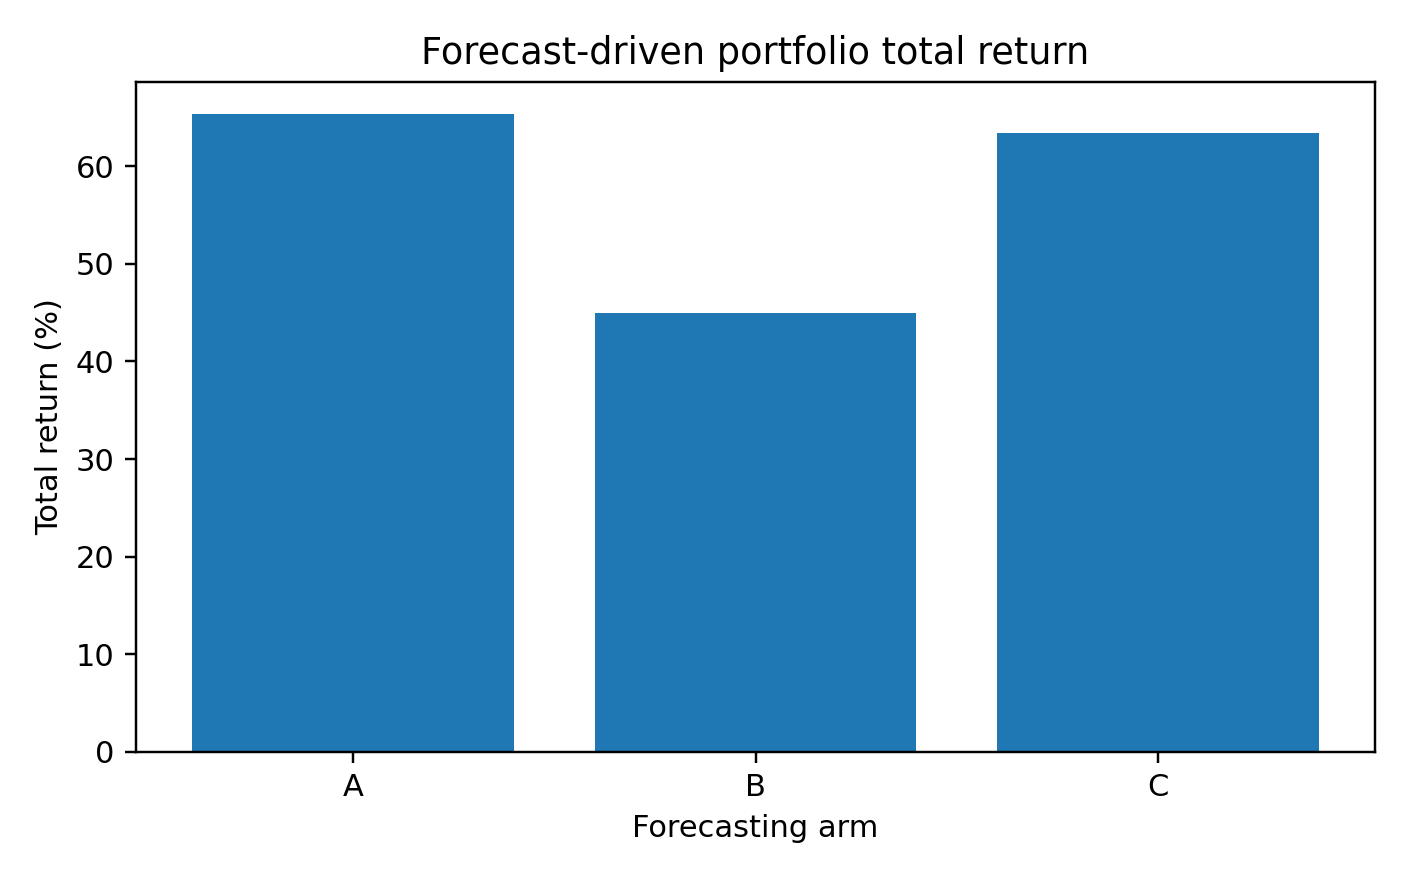
\includegraphics[width=5.8in,height=3.625in]{media/image1.png}

\emph{Figure 5.1: Total return of the forecast-driven mean-variance
portfolio by forecasting arm.}

\section{Portfolio Results}\label{portfolio-results}

\begin{longtable}{p{0.07\textwidth} p{0.13\textwidth} p{0.15\textwidth} p{0.15\textwidth} p{0.15\textwidth} p{0.13\textwidth} p{0.08\textwidth}}
\toprule
\textbf{Arm} & \textbf{Strategy} & \textbf{Total return (\%)} & \textbf{Annualized Sharpe} & \textbf{Max drawdown (\%)} & \textbf{Avg. turnover} & \textbf{Periods} \\
\midrule
\endhead
\bottomrule
\endlastfoot
A & EW & 72.43 & 1.274 & -14.74 & 0.000 & 42 \\
A & MV\_CAP & 65.36 & 1.098 & -12.76 & 1.012 & 42 \\
B & EW & 72.43 & 1.274 & -14.74 & 0.000 & 42 \\
B & MV\_CAP & 44.92 & 0.839 & -16.40 & 0.756 & 42 \\
C & EW & 72.43 & 1.274 & -14.74 & 0.000 & 42 \\
C & MV\_CAP & 63.46 & 1.050 & -16.08 & 0.962 & 42 \\
\end{longtable}

\emph{Table 5.2: Portfolio performance over 42 non-overlapping holding
periods.}

The economic comparison is more pronounced than the forecast-error
comparison. Arm A\textquotesingle s forecast-driven portfolio earns
65.36\% cumulatively with an annualized Sharpe ratio of 1.098, whereas
Arm B earns 44.92\% with a Sharpe ratio of 0.839. Arm A also has a
smaller maximum drawdown, -12.76\% versus -16.40\%. The average turnover
is higher for Arm A, so part of the improvement is achieved through more
active reallocation; transaction costs are already included in the
reported backtest.

This result directly addresses the core research question at the
descriptive level. Historical macroeconomic covariates do not merely
lower a few forecast-error metrics; they are associated with a
materially different portfolio path under the same optimizer. The Sharpe
difference of approximately 0.264 is economically visible in the sample.
The magnitude of the portfolio gap is also much larger than the
difference in average return MAE, illustrating that forecast metrics and
economic outcomes need not move proportionally.

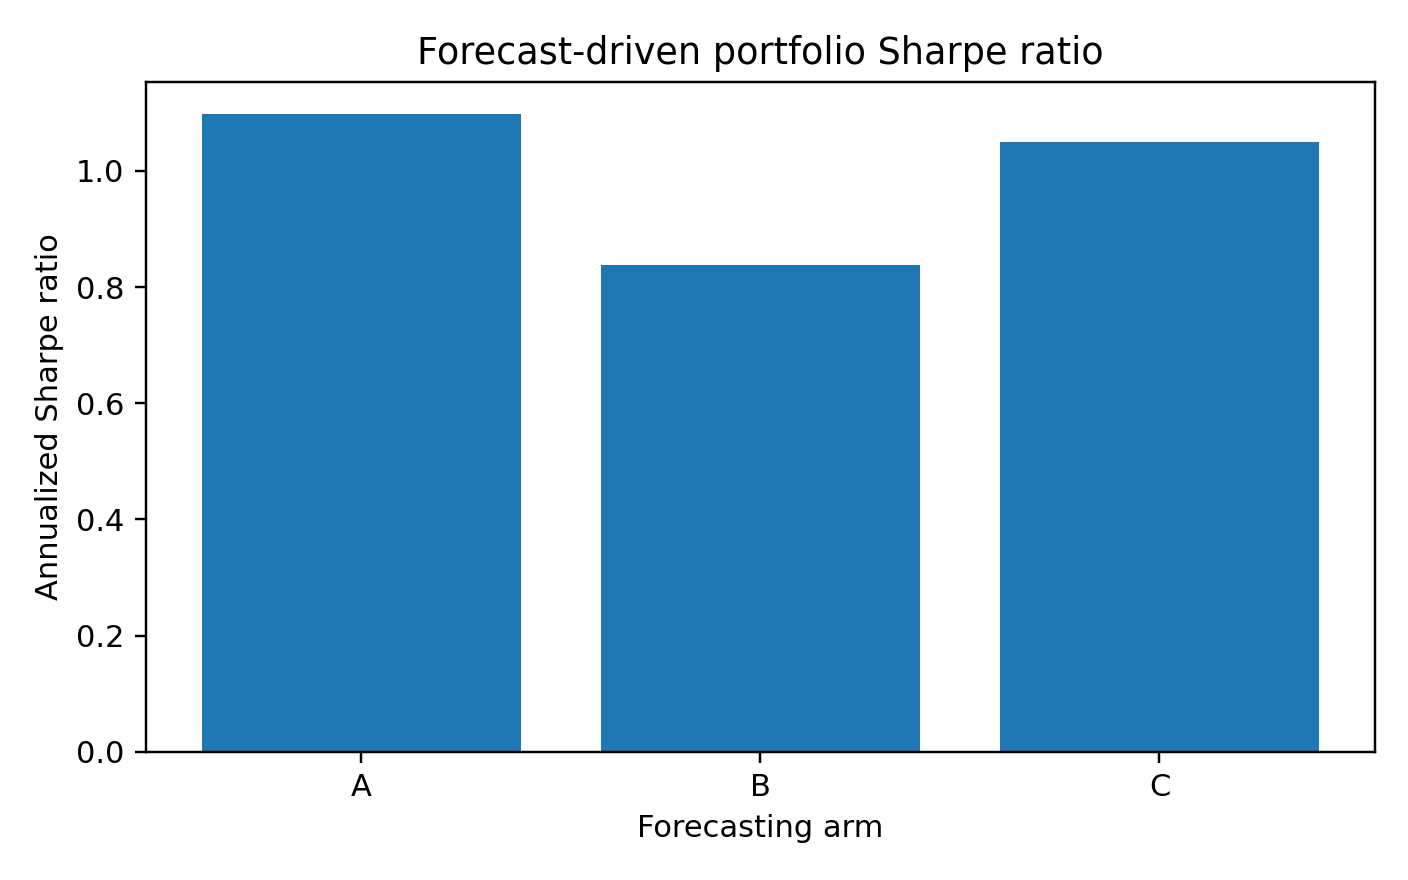
\includegraphics[width=5.8in,height=3.625in]{media/image2.png}

\emph{Figure 5.2: Annualized Sharpe ratio of the forecast-driven
portfolio by forecasting arm.}

The equal-weight benchmark is a critical counterpoint. It earns 72.43\%
with a Sharpe ratio of 1.274, exceeding all three forecast-driven
mean-variance portfolios. This prevents an overly strong interpretation
of the covariate result. Arm A is better than the Chronos-2 price-only
baseline, but the forecasting-and-optimization pipeline does not beat a
simple allocation rule in this sample. The result is therefore about the
incremental value of covariates within the chosen forecast-driven
pipeline, not about establishing a superior investment strategy.

\section{Statistical
Significance}\label{statistical-significance}

\begin{longtable}{p{0.24\textwidth} p{0.20\textwidth} p{0.28\textwidth} p{0.18\textwidth}}
\toprule
\textbf{Comparison} & \textbf{Sharpe difference} & \textbf{95\% bootstrap CI} & \textbf{Two-sided p-value} \\
\midrule
\endhead
\bottomrule
\endlastfoot
A - B & 0.264 & {[}-0.202, 0.735{]} & 0.2396 \\
C - B & 0.216 & {[}-0.284, 0.757{]} & 0.3148 \\
C - A & -0.048 & {[}-0.426, 0.413{]} & 0.8362 \\
\end{longtable}

\emph{Table 5.3: Paired circular block-bootstrap inference for
Sharpe-ratio differences.}

The bootstrap results substantially qualify the economic point
estimates. Although Arm A has a higher Sharpe ratio than Arm B, the 95\%
confidence interval ranges from -0.202 to 0.735 and therefore includes
zero. The two-sided p-value is 0.2396, well above the conventional 5\%
threshold. The correct interpretation is that the backtest shows an
economically meaningful observed improvement, but the available sample
does not provide sufficient evidence to conclude that the Sharpe
improvement is statistically reliable.

The limited number of non-overlapping periods is an important reason for
this uncertainty. Forty-two portfolio observations provide much less
inferential power than thousands of daily returns, but using overlapping
21-day outcomes as if they were independent would create a different
problem by overstating effective sample size. The non-overlapping design
and block bootstrap favor conservative inference at the cost of wider
confidence intervals.

\section{Future-Covariate
Extension}\label{future-covariate-extension}

Arm C tests whether predicted future macroeconomic paths provide
additional information beyond historical covariates. Its portfolio earns
63.46\% with a Sharpe ratio of 1.050. This is clearly above the
price-only Arm B but slightly below Arm A. The C-versus-A Sharpe
difference is -0.048 with a p-value of 0.8362, providing no evidence
that the future-covariate extension improves portfolio performance.

This result is informative even though it is not positive. Future macro
covariates are potentially powerful when they are genuinely known in
advance, as in calendar effects or scheduled promotions. In financial
markets, however, future VIX, yields, oil, gold, and dollar values are
not known and must themselves be forecast. Arm C therefore compounds two
forecasting problems. Errors in the macro forecast can propagate into
the ETF forecast, and the second-stage model may respond to predicted
macro movements that are too noisy to be useful. The result suggests
that, for this sample and implementation, historical macro context is
more useful than a recursively forecasted future macro path.

\section{Covariate Ablation}\label{covariate-ablation-1}

\begin{longtable}{p{0.26\textwidth} p{0.17\textwidth} p{0.18\textwidth} p{0.18\textwidth} p{0.15\textwidth}}
\toprule
\textbf{Specification} & \textbf{Total return (\%)} & \textbf{Annualized Sharpe} & \textbf{Max drawdown (\%)} & \textbf{Avg. turnover} \\
\midrule
\endhead
\bottomrule
\endlastfoot
All covariates & 65.36 & 1.098 & -12.76 & 1.012 \\
Without Gold & 58.85 & 1.027 & -13.85 & 0.963 \\
Without Oil & 49.32 & 0.930 & -13.53 & 1.006 \\
Without US10Y & 63.63 & 1.090 & -13.17 & 0.937 \\
Without USD & 63.43 & 1.075 & -12.93 & 1.005 \\
Without VIX & 64.29 & 1.111 & -10.78 & 0.954 \\
\end{longtable}

\emph{Table 5.4: Leave-one-covariate-out portfolio results for Arm A.}

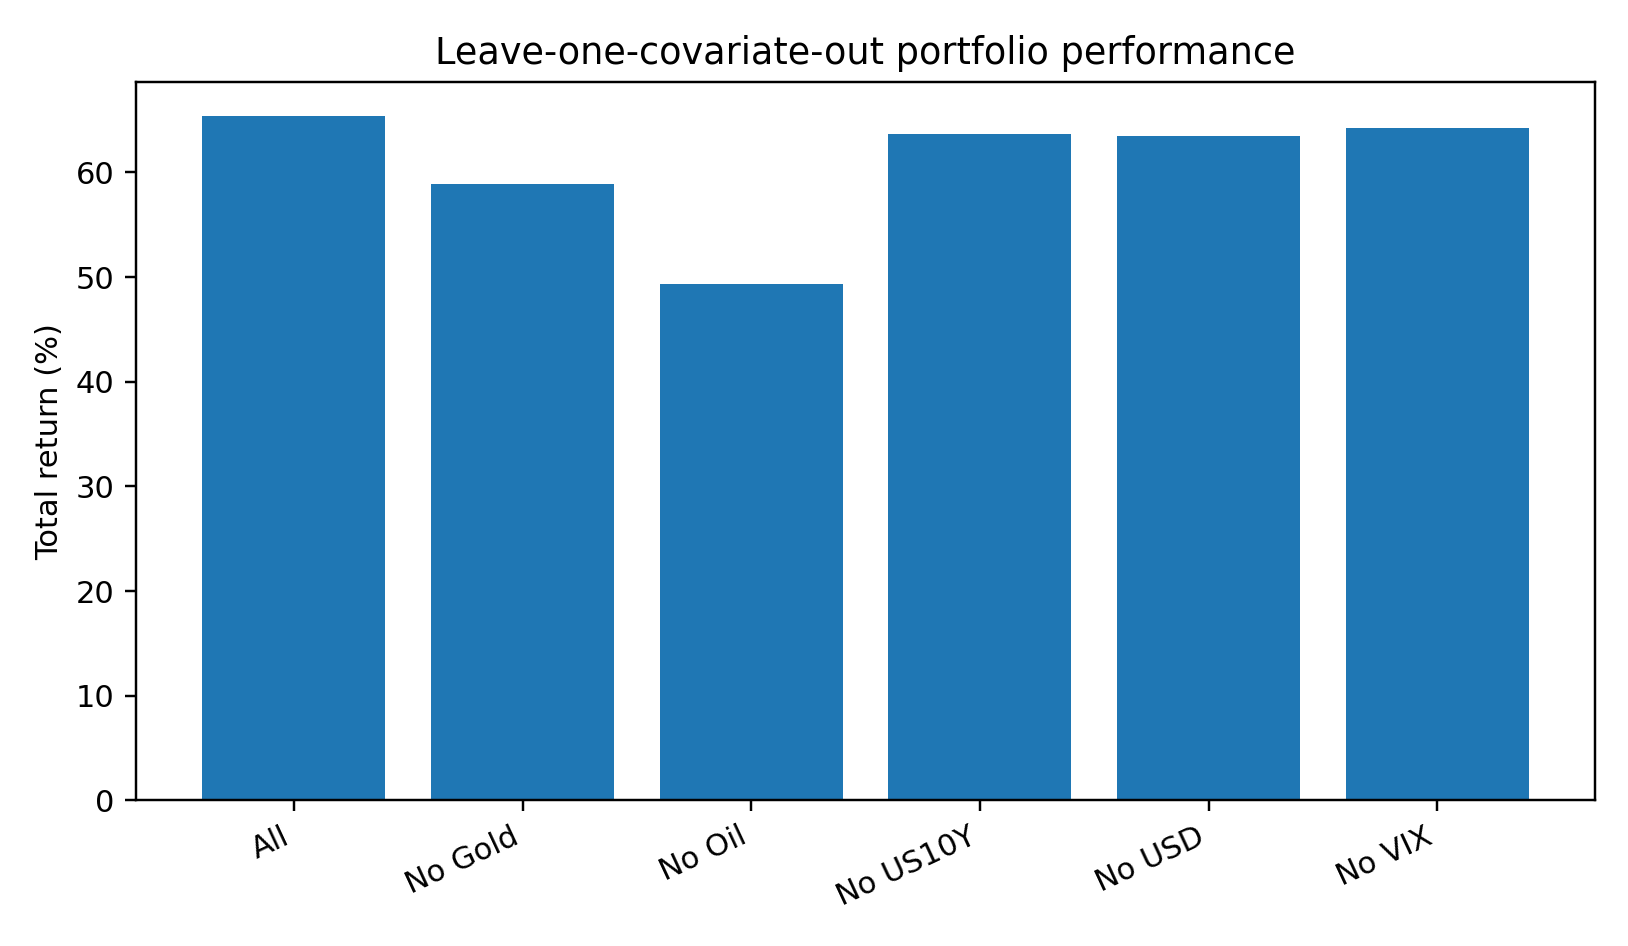
\includegraphics[width=6in,height=3.48649in]{media/image3.png}

\emph{Figure 5.3: Total return under leave-one-covariate-out ablations.}

The largest deterioration occurs when oil is removed. Total return falls
from 65.36\% to 49.32\% and the Sharpe ratio falls from 1.098 to 0.930.
Removing gold also reduces performance, producing 58.85\% total return
and a Sharpe ratio of 1.027. These changes suggest that
commodity-related information is particularly relevant to the
sector-level allocation problem in this sample.

Removing the U.S. 10-year yield or the dollar index has a smaller
effect. The corresponding Sharpe ratios are 1.090 and 1.075, close to
the full-covariate value. VIX is more ambiguous: removing it slightly
lowers total return but raises the Sharpe ratio to 1.111 and improves
maximum drawdown to -10.78\%. This is a useful reminder that a variable
can help one performance dimension while hurting another.

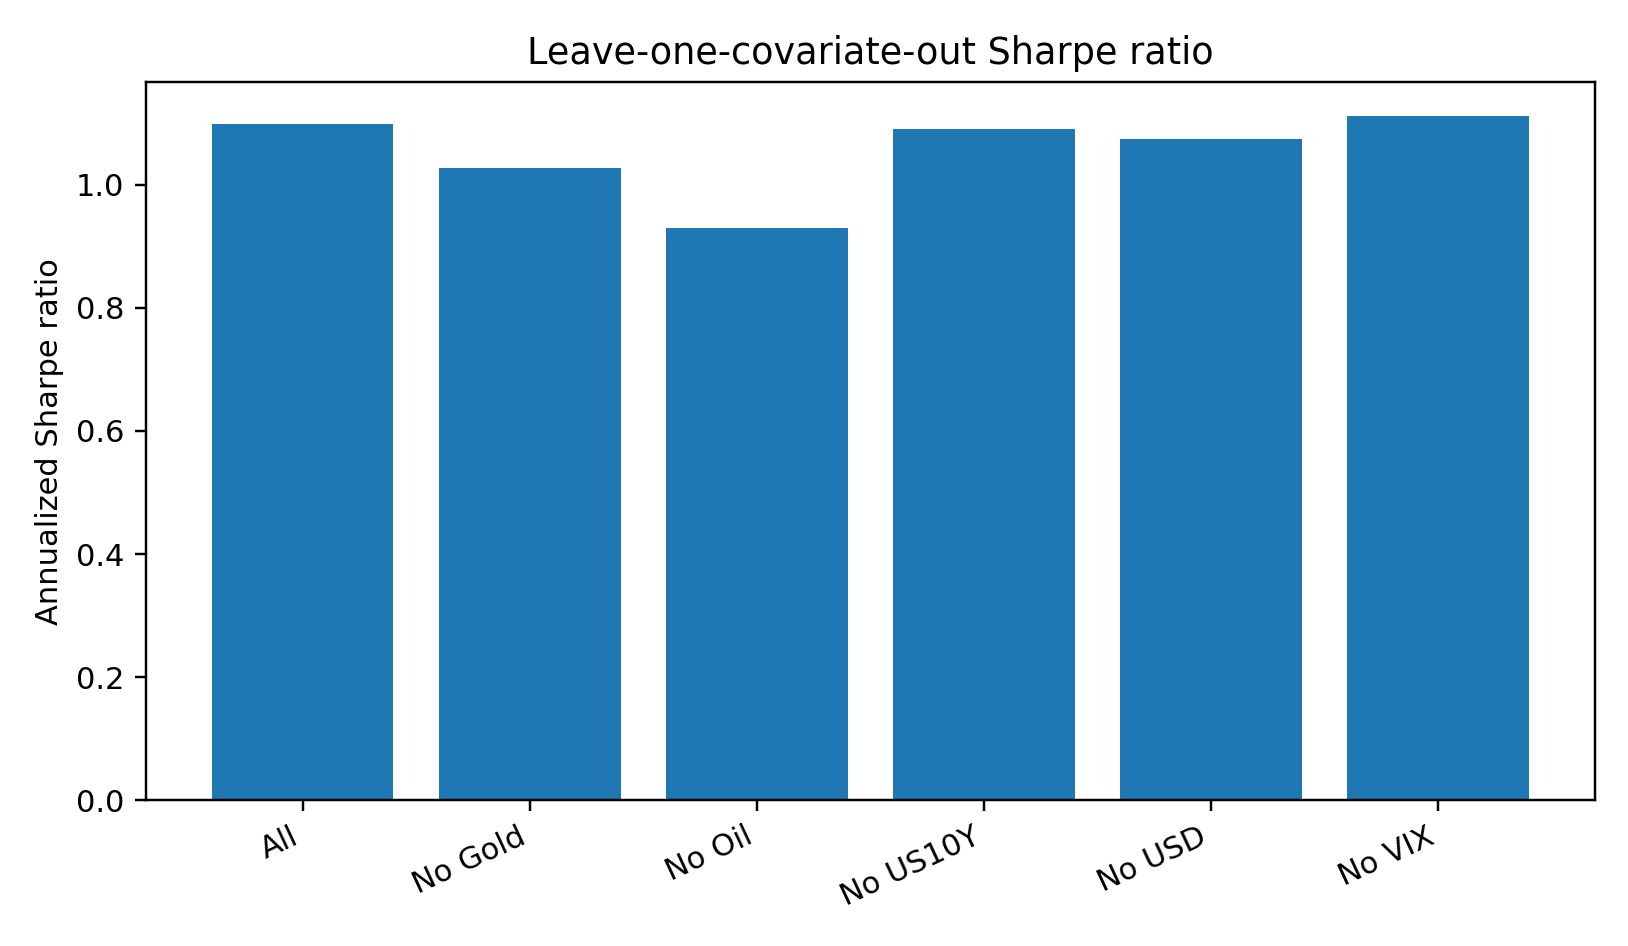
\includegraphics[width=6in,height=3.48649in]{media/image4.png}

\emph{Figure 5.4: Sharpe ratio under leave-one-covariate-out ablations.}

The forecast-level ablations reinforce the distinction between
statistical and economic importance. Removing oil changes average
forecast-error metrics only slightly, yet it has the largest portfolio
effect. Conversely, removing some variables can improve a particular
forecast metric without improving the portfolio. The optimizer responds
to the joint cross-section of expected returns, so a
covariate\textquotesingle s economic value depends on where and when it
changes relative forecasts rather than only on its average error
contribution.

\section{Statistical Accuracy versus Economic
Value}\label{statistical-accuracy-versus-economic-value}

The central empirical insight of the study is that statistical and
economic evaluation answer different questions. MAPE asks how close
predicted prices are to realized prices on average. Return MAE asks how
close predicted horizon returns are to realized returns. Directional
accuracy asks whether the sign is correct. Rank IC asks whether the
cross-sectional ordering is useful. The portfolio, in contrast, asks
whether these forecasts produce allocations that earn attractive
realized returns after risk constraints and costs.

Arm A illustrates this separation. Its forecast improvements over B are
small in percentage terms, but its portfolio improvement is large. One
plausible mechanism is that the covariates alter the relative ranking or
magnitude of forecasts at economically important decision dates. Arm C
provides the opposite caution: it has the strongest rank IC and the best
return MAE, yet its portfolio does not beat Arm A. Portfolio performance
depends on the entire interaction among expected returns, covariance,
constraints, turnover, and realized market outcomes.

This finding supports the motivation for evaluating forecasting models
in the context of the decision they are intended to support. A
forecasting paper that stops at average error can miss economically
relevant changes, while a portfolio paper that reports only Sharpe
ratios can obscure whether gains arise from better forecasts or from
other elements of the pipeline. The controlled design used here makes
both layers visible.

\section{Limitations and
Robustness}\label{limitations-and-robustness}

The first limitation is sample size. The final inference is based on 42
non-overlapping 21-trading-day periods. This is appropriate for avoiding
overlapping-horizon dependence, but it produces wide uncertainty around
Sharpe differences. Extending the historical sample would increase
power, although older data can also introduce regime changes and
data-availability complications.

Second, the study uses one foundation model and one portfolio rule. The
conclusion should therefore be stated as a result about Chronos-2 within
this controlled mean-variance pipeline, not as a universal statement
about all foundation models or all optimization methods. Alternative
risk models, turnover penalties, robust optimization, or direct ranking
strategies could transform the same forecasts differently.

Third, the macro variables are economically plausible but not
exhaustive. Other variables such as credit spreads, inflation
expectations, liquidity measures, or sector-specific fundamentals may
provide different information. The ablation results also do not
establish causality: removing oil changes the model\textquotesingle s
information set, but the observed portfolio deterioration may depend on
interactions with the remaining covariates and the specific market
regime.

Fourth, Arm C uses model-generated future covariates rather than
historically archived real-time forecasts of macro variables. This is
necessary to avoid look-ahead bias, but it means the experiment tests a
recursive forecasting design. A stronger future-covariate test could use
information that was genuinely known at each decision date, such as
scheduled macro announcements, futures-implied measures, or archived
consensus forecasts.

Finally, the equal-weight result is a meaningful benchmark challenge.
The fact that equal weight outperforms the forecast-driven strategies
suggests that estimation error and optimization sensitivity remain
important. Future work should therefore investigate whether the
covariate information is better exploited through more robust portfolio
mappings rather than assuming that improved forecasts should
automatically be fed into a standard mean-variance optimizer.

\chapter{Conclusion}\label{conclusion}

\section{Summary}\label{summary}

This research asked whether macroeconomic covariates improve the
economic value of zero-shot Chronos-2 forecasts in a multi-asset
portfolio setting. The study compared a price-only baseline with a
historical-covariate treatment and a future-covariate extension across
11 U.S. sector ETFs. The experimental design aligned the information
cutoff, 21-trading-day forecast horizon, expected-return definition, and
realized portfolio holding period, and held the portfolio optimizer
fixed across arms.

The results provide qualified support for the usefulness of historical
macroeconomic covariates. Arm A improves several forecast-error measures
relative to Arm B and produces a substantially stronger observed
mean-variance portfolio: 65.36\% cumulative return and a Sharpe ratio of
1.098 versus 44.92\% and 0.839. However, the block-bootstrap p-value of
0.2396 and a confidence interval spanning zero mean that the Sharpe
improvement is not statistically conclusive. The simple equal-weight
benchmark also remains superior in return and Sharpe ratio.

The future-covariate extension does not improve on historical covariates
alone. Arm C remains stronger than the no-covariate baseline in observed
portfolio performance but slightly weaker than Arm A. The ablation
analysis suggests that oil and gold are particularly associated with the
portfolio improvement, while the yield, dollar, and VIX effects are
smaller or depend on the metric considered.

\section{Implications}\label{implications}

The main implication is methodological. Foundation-model forecasting
should be evaluated at both the statistical and decision levels.
Covariates can change the economic behavior of a forecasting pipeline
even when average forecast metrics move only modestly. At the same time,
an economically attractive backtest difference should not be treated as
established evidence when uncertainty is large. Reporting forecast
errors, portfolio metrics, simple benchmarks, and formal inference
together produces a more credible assessment.

For practitioners, the results suggest that historical macro context can
be worth testing when using a flexible zero-shot forecaster across
related assets. But additional information should not be assumed to
help: noisy future covariate forecasts can fail to add value, and
individual covariates can have heterogeneous effects. The equal-weight
benchmark further shows that model sophistication does not guarantee
superior allocation.

\section{Future Work}\label{future-work}

Several extensions follow naturally. A longer historical evaluation
could improve statistical power and allow subperiod analysis across
market regimes. Alternative portfolio mappings could test whether robust
optimization, rank-based allocation, minimum-variance anchors, or
explicit turnover regularization better convert forecast information
into economic value. The covariate set could be expanded to include
credit, inflation, liquidity, and sector-specific variables.

A particularly important extension is decision-focused or end-to-end
training. The present study intentionally uses predict-then-optimize so
that the marginal role of covariates can be isolated. Recent Smart
Predict-then-Optimize research shows how forecasting models can instead
be trained against downstream portfolio objectives. Comparing the
controlled two-stage design with an end-to-end objective would test
whether covariate information becomes more useful when the model is
explicitly rewarded for decision quality rather than forecast accuracy.

Finally, future-covariate research should distinguish variables that are
truly known ahead of time from variables that must themselves be
forecast. Archived real-time macro expectations, futures curves,
scheduled events, and survey forecasts could provide more realistic
future information. Such work would clarify when
Chronos-2\textquotesingle s future-covariate interface offers genuine
financial value rather than simply adding another noisy prediction
layer.

\chapter*{Bibliography}\addcontentsline{toc}{chapter}{Bibliography}

Ansari, A. F., Shchur, O., Küken, J., et al. (2025). Chronos-2: From
univariate to universal forecasting. Amazon Science / Chronos-2
technical materials.

Arango, S. P., Mercado, P., Kapoor, S., Ansari, A. F., Stella, L., Shen,
H., et al. (2025). ChronosX: Adapting pretrained time series models with
exogenous variables. Proceedings of AISTATS 2025; arXiv:2503.12107.

Das, S. R., Goyal, T., \& Yadav, M. (2026). Multivariate Financial
Forecasting using the Chronos Time Series Foundation Models.
arXiv:2605.21504.

Engel, R., Chen, Y., Polak, P., \& Boier, I. (2025). Scaling Conditional
Autoencoders for Portfolio Optimization via Uncertainty-Aware Factor
Selection. Proceedings of the 6th ACM International Conference on AI in
Finance, 123-131. https://doi.org/10.1145/3768292.3770415.

Gu, S., Kelly, B., \& Xiu, D. (2020). Empirical Asset Pricing via
Machine Learning. Review of Financial Studies, 33(5), 2223-2273.
https://doi.org/10.1093/rfs/hhaa009.

Markowitz, H. (1952). Portfolio Selection. Journal of Finance, 7(1),
77-91.

Noguer i Alonso, M., \& Franklin, R. P. (2026). Pretrained Time-Series
Foundation Models for Financial Return Forecasting. arXiv:2606.27100.

Pishehvar, R. (2026). A Three-Phase Foundation Model for Tax-Aware
Personalized Portfolio Management. arXiv:2606.30997.

Tire, {[}authors as in published record{]}. (2026). End-to-end portfolio
selection: Leveraging deep learning in Smart Predict then Optimize.
Computers \& Operations Research, article 107638.
https://doi.org/10.1016/j.cor.2026.107638.

Valeyre, S., \& Aboura, S. (2024/2025). LLMs for Time Series: an
Application for Single Stocks and Statistical Arbitrage.
arXiv:2412.09394.

Welch, I., \& Goyal, A. (2008). A Comprehensive Look at the Empirical
Performance of Equity Premium Prediction. Review of Financial Studies,
21(4), 1455-1508. https://doi.org/10.1093/rfs/hhm014.

Amazon Science. (2025). Introducing Chronos-2: From univariate to
universal forecasting.

Amazon Science. (2026). Impact-driven event covariates for time-series
foundation models.

Buonanno, A., Fabozzi, S., Valenti, M., \& Graditi, G. (2026). The
Impact of Covariates on Zero-Shot Building Energy Forecasting Using
Chronos-2 Foundation Model. Electronics, 15(15), 3474.

\section{Appendix A: Reproduction
Commands}\label{appendix-a-reproduction-commands}

The final V3 pipeline can be reproduced from the repository root with
the following commands:

python src\_v3/forecast.py

python src\_v3/forecast\_armA.py

python src\_v3/forecast\_armC.py

python src\_v3/evaluate.py

python src\_v3/portfolio.py

python src\_v3/significance.py

python src\_v3/forecast\_ablations.py

python src\_v3/evaluate\_ablations.py

python src\_v3/portfolio\_ablations.py

python src\_v3/make\_figures.py

Arm B is generated by forecast.py, Arm A by forecast\_armA.py, and Arm C
by forecast\_armC.py. The ablation scripts repeat Arm A while removing
one macro covariate at a time. Summary outputs are stored in
results\_v3, while large forecast-level CSV files may be excluded from
version control because they can be regenerated.

\section{Appendix B: Additional Result
Tables}\label{appendix-b-additional-result-tables}

\subsection{B.1 Forecast Ablations}\label{b.1-forecast-ablations}

\begin{longtable}{p{0.18\textwidth} p{0.12\textwidth} p{0.13\textwidth} p{0.12\textwidth} p{0.12\textwidth} p{0.16\textwidth} p{0.10\textwidth}}
\toprule
\textbf{Specification} & \textbf{Median MAPE} & \textbf{Quantile loss} & \textbf{Return MAE} & \textbf{Return RMSE} & \textbf{Directional acc.} & \textbf{Rank IC} \\
\midrule
\endhead
\bottomrule
\endlastfoot
A & 2.957 & 1.262 & 3.976 & 5.297 & 49.57 & 0.050 \\
A without Gold & 2.983 & 1.268 & 3.970 & 5.298 & 50.43 & 0.029 \\
A without Oil & 2.919 & 1.261 & 3.971 & 5.306 & 48.92 & 0.016 \\
A without US10Y & 2.898 & 1.261 & 3.974 & 5.302 & 49.35 & 0.057 \\
A without USD & 2.955 & 1.262 & 3.971 & 5.288 & 48.48 & 0.079 \\
A without VIX & 3.010 & 1.269 & 4.028 & 5.377 & 52.16 & 0.070 \\
\end{longtable}

The table shows why no single covariate can be labeled universally
\textquotesingle best\textquotesingle. Removing VIX worsens return MAE
but improves directional accuracy and rank IC. Removing oil leaves
average forecast errors close to the full model but materially weakens
the downstream portfolio. These mixed patterns motivate a decision-level
analysis.

\subsection{B.2 Interpretation Guide}\label{b.2-interpretation-guide}

For MAPE, quantile loss, return MAE, and return RMSE, lower values
indicate smaller errors. For directional accuracy and rank IC, higher
values indicate better sign or cross-sectional ordering. Portfolio total
return and Sharpe ratio are evaluated together with drawdown and
turnover; a higher return is not automatically preferable if it is
obtained with disproportionate risk or trading.


\end{document}
